%% Recipes_Detector.tex
%% Created:     Tue Apr  4 16:37:17 2017 by Koehler@I-Mac
%% Last change: 2020-09-04
%%
%% subsection for Detector Recipes
%%
%%%%%%%%%%%%%%%%%%%%%%%%%%%%%%%%%%%%%%%%%%%%%%%%%%%%%%%%%%%%%%%%%%%%%%%%%%%%%
\subsection{Detector calibration recipes}
\label{Sec:detector_calibration}

METIS will have three focal plane detector arrays:
\begin{itemize}
\item One $2\mathrm{k}\times 2\mathrm{k}$ HAWAII2RG detector used for
  LM-band imaging and slit spectroscopy.
\item One $2\mathrm{k}\times 2\mathrm{k}$ GeoSnap (Teledyne) detector
  used for N-band imaging and slit spectroscopy.
\item An array of four $2\mathrm{k}\times 2\mathrm{k}$ HAWAII2RG
  detectors used for LM-band integral-field spectroscopy.
\end{itemize}
This section lists recipes that calibrate detector characteristics
independent of a specific instrument mode. Where \FITS{_det} appears
in FITS keywords of input or product files, it is taken to mean
\FITS{_LM}, \FITS{_N} or \FITS{_IFU} according to the detector
array for which data are being processed.

\subsubsection{Detector linearity and gain determination recipe \REC{metis_det_lingain}}
\label{sssec:metis_det_lingain}
\label{rec:metis_det_lingain}
\label{rec:metisdetlingain}

The recipe \hyperref[rec:metis_det_lingain]{\REC{metis_det_lingain}} determines detector (non-)linearity and absolute detector
gain from a set of flat-field frames taken with the broad-band lamp
over a range of detector exposure times (DITs) and flux levels. The
recipe structure will be similar as for \CODE{detmon_ir_lg} % Not a \REC because it is not our recipe
\cite{detmon-manual}; however, further insight into detector behaviour
(in particular of GeoSnap) may necessitate development of more complex
procedures.

The linearity curve is given by the measured background level as a
function of exposure time for constant illumination. For each pixel
the coefficients of a polynomial fit (order TBD) will be recorded in a
coefficient cube, which can in turn be used to correct for
non-linearity in other recipes. Pixels whose coefficients differ
significantly from the majority of pixels will be marked as bad.

Detector gain is typically computed pixelwise as the slope of a linear
fit of the variance against the mean (or median) values over a set of
frames taken over a range of DITs and illumination levels.  For
mid-infrared detectors that suffer from \ac{ELFN}, e.g.\ the AQUARIUS
detector, this approach does not work.  The GeoSnap is not expected to
show \ac{ELFN}, hence gain determination is probably possible.

The set of calibration frames used for this recipes will include
exposures with WCU window closed (\CODE{LAMP OFF}), which will be used
as `dark' frames that captur thermal emission within the
instrument. This is subtracted from all other exposures in the
sequence.

This satisfies \REQ{METIS-5997}.

\newpage
\begin{recipedef}
  Name:                & \hyperref[rec:metis_det_lingain]{\REC{metis_det_lingain}}                                                             \\
  Purpose:             & determine non-linearity and gain of the detectors                                   \\
  Requirements:        & \REQ{METIS-5997}                                                                    \\
  Type:                & Calibration                                                                         \\
  Templates:           & \TPL{METIS_img_lm_cal_DetLin}                                                       \\
                       & \TPL{METIS_img_n_cal_DetLin}                                                        \\
                       & \TPL{METIS_ifu_cal_DetLin}                                                          \\
  Input data:          & \hyperref[dataitem:detlin_det_raw]{\RAW{DETLIN_det_RAW}}: (set of \FITS{FLAT,LAMP} frames taken with increasing DIT) \\
                       & \hyperref[dataitem:det_wcu_off_raw]{\RAW{det_WCU_OFF_RAW}}: (set of internal darks taken at the start of the template) \\
 % Matched keywords:    & Subsystem ID \TODO{TBD}                                                             \\
  Algorithm:           & Subtract instrument dark (\CODE{hdrl_imagelist_sub_image}).                         \\
                       & Compute mean and variance for each frame (\CODE{TBD}).                              \\
                       & Gain is determined as the slope of variance against mean (\hyperref[drl:metis_derive_gain]{\DRL{metis_derive_gain}}) \\
                       & Fit polynomial of value as a function of DIT and illumination level for each pixel (\hyperref[drl:metis_derive_nonlinearity]{\CODE{metis_derive_nonlinearity}}). \\
                       & Flag pixels with coefficients significantly different from the mean of all pixels. (\CODE{hdrl_bpm_fit_compute}) \\
  Output data:         & \hyperref[dataitem:gain_map_det]{\PROD{GAIN_MAP_det}}                                    \\
                       & \hyperref[dataitem:linearity_det]{\PROD{LINEARITY_det}}                                 \\
                       & \hyperref[dataitem:badpix_map_det]{\PROD{BADPIX_MAP_det}}                                \\
  Expected accuracies: & 0.5\% background subtraction (cf. \cite{METIS_calerrbudget})                             \\
                       & 0.1\% non-linearity measurement (cf. \cite{METIS_calerrbudget})                          \\
  QC1 parameters:      & \hyperref[qc:qc_lin_gain_mean]{\QC{QC LIN GAIN MEAN}}                                    \\
                       & \hyperref[qc:qc_lin_gain_rms]{\QC{QC LIN GAIN RMS}}                                      \\
                       & \hyperref[qc:qc_lin_num_badpix]{\QC{QC LIN NUM BADPIX}}                                  \\
  hdrl functions:      & \CODE{hdrl_imagelist_sub_image}                                                     \\
                       & \CODE{hdrl_bpm_fit_compute}                                                         \\
\end{recipedef}

\begin{figure}[hb]
  \centering
    \begingroup
        \def \globalscale {0.700000}
        \fontsize{10}{12}\selectfont
        % % Document preamble. Comment out for final figure! Footer too!
% \documentclass[tikz, margin=5mm, dvipsnames]{standalone}
% \usepackage{listings}
% 
% ADDING NEW DEFINITIONS -------------------------------------------- start
\definecolor{listingbg}{gray}{0.95}
\definecolor{darkgreen}{rgb}{0.0, 0.7, 0.0}
\definecolor{darkblue} {rgb}{0.0, 0.0, 0.7}
\definecolor{cyan} {rgb}{0.0, 0.4, 0.4}
\definecolor{darkred}  {rgb}{0.7, 0.0, 0.0}
\definecolor{darkorange}{rgb}{1.0, 0.49, 0.0}
\definecolor{violett}{rgb}{255, 0, 255}
\definecolor{turq}{rgb}{0.0, 0.7, 0.8}
\definecolor{fits}{rgb}{0.4, 0.1, 1}


\makeatletter
\lstdefinestyle{RAWstyle}{%
  basicstyle=\ttfamily\color{black}%
  \lst@ifdisplaystyle\scriptsize\fi}

\lstdefinestyle{PARstyle}{%
  basicstyle=\ttfamily\color{black}%
  \lst@ifdisplaystyle\scriptsize\fi}

\lstdefinestyle{DRLstyle}{%
  basicstyle=\ttfamily\color{black}%
  \lst@ifdisplaystyle\scriptsize\fi}

\lstdefinestyle{RECstyle}{%
  basicstyle=\ttfamily\color{black}%
  \lst@ifdisplaystyle\scriptsize\fi}

\lstdefinestyle{QCstyle}{%
  basicstyle=\ttfamily\color{black}%
  \lst@ifdisplaystyle\scriptsize\fi}

\lstdefinestyle{TPLstyle}{%
  basicstyle=\ttfamily\color{black}%
  \lst@ifdisplaystyle\scriptsize\fi}

\lstdefinestyle{PRODstyle}{%
  basicstyle=\ttfamily\color{black}%
  \lst@ifdisplaystyle\scriptsize\fi}

\lstdefinestyle{EXTCALIBstyle}{%
  basicstyle=\ttfamily\color{black}%
  \lst@ifdisplaystyle\scriptsize\fi}

\lstdefinestyle{STATCALIBstyle}{%
  basicstyle=\ttfamily\color{black}%
  \lst@ifdisplaystyle\scriptsize\fi}
\makeatother

% \makeatletter
\newcommand{\replaceunderscores}[1]{\expandafter\replace@underscores#1_\relax}

\def\replace@underscores#1_#2\relax{%
    \ifx \relax #2\relax
        #1%
    \else
        #1%
        \textunderscore
        \replace@underscores#2\relax
    \fi
}

\ExplSyntaxOn
% Generic \Smart@Item macro:
%   use \NEWRAW*{WHATEVER_THIS_IS} where hyperlinks are not needed (TOC, sections...)
%   and \NEWRAW{WHATEVER_THIS_IS} for a full hyperlink-enabled version in regular text and tikz figures
\NewDocumentCommand{\Smart@Item}{m m m O{dataitem}}{%
    \IfBooleanTF{#1}{%
        \texorpdfstring{\lstinline[style=#2style]!#3!}{\replaceunderscores{#3}}%
    }{%
        \hyperref[#4:\text_lowercase:n{#3}]{\lstinline[style=#2style]!#3!}%
    }%
}
\ExplSyntaxOff

% Raw FITS file: \NEWRAW{LM_SCI_RAW}
\NewDocumentCommand{\NEWRAW}{s m}{\Smart@Item{#1}{RAW}{#2}}
\NewDocumentCommand{\NEWPAR}{s m}{\Smart@Item{#1}{PAR}{#2}}
\NewDocumentCommand{\NEWDRL}{s m}{\Smart@Item{#1}{DRL}{#2}}
\NewDocumentCommand{\NEWREC}{s m}{\Smart@Item{#1}{REC}{#2}[rec]}
\NewDocumentCommand{\NEWQC}{s m}{\Smart@Item{#1}{QC}{#2}}
\NewDocumentCommand{\NEWTPL}{s m}{\Smart@Item{#1}{TPL}{#2}}
\NewDocumentCommand{\NEWPROD}{s m}{\Smart@Item{#1}{PROD}{#2}}
\NewDocumentCommand{\NEWREQ}{s m}{\Smart@Item{#1}{REQ}{#2}}
\NewDocumentCommand{\NEWEXTCALIB}{s m}{\Smart@Item{#1}{EXTCALIB}{#2}}
\NewDocumentCommand{\NEWSTATCALIB}{s m}{\Smart@Item{#1}{STATCALIB}{#2}}
\NewDocumentCommand{\NEWFITS}{s m}{\Smart@Item{#1}{FITS}{#2}}
\makeatother

%% Write DRL functions names like this: \hyperref[drl:function]{\DRL{function}}
\newcommand{\RAW}[1]{ \texorpdfstring{\lstinline[style=RAWstyle]!#1!}%
                                     {\replaceunderscores{#1}}}

%% Write DRL functions names like this: \hyperref[drl:function]{\DRL{function}}
\newcommand{\PAR}[1]{ \texorpdfstring{\lstinline[style=PARstyle]!#1!}%
                                     {\replaceunderscores{#1}}}

%% Write DRL functions names like this: \hyperref[drl:function]{\DRL{function}}
\newcommand{\DRL}[1]{ \texorpdfstring{\lstinline[style=DRLstyle]!#1!}%
                                     {\replaceunderscores{#1}}}

%% Write recipe names like this: \REC{metis_do_stuff}
\newcommand{\REC}[1]{ \texorpdfstring{\lstinline[style=RECstyle]!#1!}%
                                     {\replaceunderscores{#1}}}

%% Write QC parameters like this: \QC{QC_SOMETHING_OR_OTHER}
\newcommand{\QC}[1]{ \texorpdfstring{\lstinline[style=QCstyle]!#1!}%
                                    {\replaceunderscores{#1}}}

%% Write templates like this: \TPL{DARK_LM}
\newcommand{\TPL}[1]{ \texorpdfstring{\lstinline[style=TPLstyle]!#1!}%
                                     {\replaceunderscores{#1}}}

%% Write products like this: \hyperref[dataitem:some_thing]{\PROD{SOME_THING}}
\newcommand{\PROD}[1]{ \texorpdfstring{\lstinline[style=PRODstyle]!#1!}%
                                      {\replaceunderscores{#1}}}

%% Write requirements like this: \REQ{METIS-xxxx}
\newcommand{\REQ}[1]{\href{https://polarion.astron.nl/polarion/\#/project/METIS/workitem?id=#1}{\textcolor{brown}{#1}}}

%% external calib files
\newcommand{\EXTCALIB}[1]{ \texorpdfstring{\lstinline[style=EXTCALIBstyle]!#1!}%
                                          {\replaceunderscores{#1}}}

% static calib files
\newcommand{\STATCALIB}[1]{ \texorpdfstring{\lstinline[style=STATCALIBstyle]!#1!}%
                                           {\replaceunderscores{#1}}}

%% Write FITS keywords (and values) like this: \FITS{EXPTIME}
\newcommand{\FITS}[1]{ \texorpdfstring{\lstinline[]!#1!}%
                                      {\replaceunderscores{#1}}}


% \begin{document}


% ADDING NEW DEFINITIONS -------------------------------------------- start
\definecolor{listingbg}{gray}{0.95}
\definecolor{darkgreen}{rgb}{0.0, 0.7, 0.0}
\definecolor{darkblue} {rgb}{0.0, 0.0, 0.7}
\definecolor{cyan} {rgb}{0.0, 0.4, 0.4}
\definecolor{darkred}  {rgb}{0.7, 0.0, 0.0}
\definecolor{darkorange}{rgb}{1.0, 0.49, 0.0}
\definecolor{violett}{rgb}{255, 0, 255}
\definecolor{turq}{rgb}{0.0, 0.7, 0.8}
\definecolor{fits}{rgb}{0.4, 0.1, 1}


\makeatletter
\lstdefinestyle{RAWstyle}{%
  basicstyle=\ttfamily\color{black}%
  \lst@ifdisplaystyle\scriptsize\fi}

\lstdefinestyle{PARstyle}{%
  basicstyle=\ttfamily\color{black}%
  \lst@ifdisplaystyle\scriptsize\fi}

\lstdefinestyle{DRLstyle}{%
  basicstyle=\ttfamily\color{black}%
  \lst@ifdisplaystyle\scriptsize\fi}

\lstdefinestyle{RECstyle}{%
  basicstyle=\ttfamily\color{black}%
  \lst@ifdisplaystyle\scriptsize\fi}

\lstdefinestyle{QCstyle}{%
  basicstyle=\ttfamily\color{black}%
  \lst@ifdisplaystyle\scriptsize\fi}

\lstdefinestyle{TPLstyle}{%
  basicstyle=\ttfamily\color{black}%
  \lst@ifdisplaystyle\scriptsize\fi}

\lstdefinestyle{PRODstyle}{%
  basicstyle=\ttfamily\color{black}%
  \lst@ifdisplaystyle\scriptsize\fi}

\lstdefinestyle{EXTCALIBstyle}{%
  basicstyle=\ttfamily\color{black}%
  \lst@ifdisplaystyle\scriptsize\fi}

\lstdefinestyle{STATCALIBstyle}{%
  basicstyle=\ttfamily\color{black}%
  \lst@ifdisplaystyle\scriptsize\fi}
\makeatother

%%% This file contains definitions of shapes and nodes used
%%% for a recipe workflow
%%% Author       : Oliver Czoske
%%% Created      : 2021-03-03
%%% Last Changed : 2021-03-03
%%% Changes:
%%%

\usetikzlibrary{
  shapes.misc,
  positioning,
  calc,
  arrows.meta}

%% All connecting lines have an arrow
\tikzset{
  connection_arrow/.style={->, >=Latex[open], thick}
}

%% Start and stop buttons (black disks, stop with ring)
%% These are pics, use as
%%         \pic (name) [above of=..] {picname};
\tikzset{
  start/.pic = {
    \node (-m) at (0, 0){};
    \filldraw [fill=black] (0, 0) circle (0.2);
  }
}

\tikzset{
  stop/.pic = {
    \node (-m) at (0, 0){};
    \node (-t) at (0, -0.3){};
    \filldraw [fill=black] (0, 0) circle(0.2);
    \draw[black] (0, 0) circle (0.3);
  }
}


%%%% Various boxes and their colours
%%%% These are nodes, use as
%%%% \node (name) [type, location]  {text};

\definecolor{stepcolor}{RGB}{210,169,188}
\definecolor{rawcolor}{RGB}{205,205,205}
\definecolor{externalcolor}{RGB}{183,255,255}
\definecolor{calibcolor}{RGB}{255,250,216}
\definecolor{calproductcolor}{RGB}{185,184,237}
\definecolor{qcproductcolor}{RGB}{255,201,165}
\definecolor{sciproductcolor}{RGB}{197,219,183}
\definecolor{framecolor}{RGB}{127,13,65}

\tikzset{
  %% template : the template(s) that trigger(s) the recipe
  template/.style={
    rectangle,
    draw=black,
    minimum width=4.0cm,
    minimum height=0.5cm,
    align=center
  },
  %% input : the input files
  input/.style={
    rectangle,
    fill=rawcolor,
    minimum width=4.0cm,
    minimum height=0.75cm,
%     text width=3cm,
    align=center
  },
  %% calib : calibration input
  calib/.style={
    rectangle,
    fill=calibcolor,
    minimum width=4.0cm,
    minimum height=0.75cm,
%     text width=3cm,
    align=center
  },
  %% external : external input
  external/.style={
    rectangle,
    fill=externalcolor,
    minimum width=4.0cm,
    minimum height=0.75cm,
%     text width=3.5cm,
    align=center
  },
  %% params : parameters
  params/.style={
    rectangle,
    draw=red,
    thick,
    minimum width=4.0cm,
    minimum height=0.75cm,
%     text width=3cm,
    align=center
  },
  %% redstep : a reduction step
  %%      ("step" is predefined and can't be used)
  redstep/.style={
    rectangle,
    rounded corners=0.2cm,
    fill=stepcolor,   %%% define colour!
    minimum width=4.0cm,
    minimum height=1cm,
%     text width=3cm,
    align=center
  },
  %% connection : connection to input or output
  connection/.style={
    circle,
    fill=black,
    minimum size=0.15cm,
    inner sep=0pt
  },
  %% sciproduct : a science product
  sciproduct/.style={
    rectangle,
    fill=sciproductcolor,
    minimum width=4.0cm,
    minimum height=0.75cm,
%     text width=3.5cm,
    align=center
  },
  %% calproduct : a calibration product
  calproduct/.style={
    rectangle,
    fill=calproductcolor,
    minimum width=4.0cm,
    minimum height=0.75cm,
%     text width=3.5cm,
    align=center
  },
  %% frame : frame around the recipe
  %% This is a path, use as
  %%    \draw [frame] (upper left) rectangle (lower right);
  frame/.style={framecolor, very thick, dashed}
}



\begin{tikzpicture}
  [x=1cm,
  y=-1cm,
  align=center,
  node distance=2cm and 3.5cm]
  \sffamily

%   % Grid for orientation. Comment out for final figure!
%   \draw[help lines, green](-5, 0) grid (8, 11);

  %%% Put workflow commands here:
  %% Main reduction workflow

  \node (template) [template]{%
    \TPL{METIS\_img\_lm\_cal\_DetLin}\\
    \TPL{METIS\_img\_n\_cal\_DetLin}\\
    \TPL{METIS\_ifu\_cal\_DetLin}};

  \pic (start) [below=0.75cm of template] {start};

  \node (input) [below=0.75cm of start-m, input] {%
    \textsl{N} \RAW{DETLIN_det_RAW}\\
    \RAW{det_WCU_OFF_RAW}};

  \node (step_persistence) [below=2.0cm of input, redstep] {%
    apply persistence correction};

  \node (step_dark) [below of=step_persistence, redstep]{%
    subtract dark};

  \node (step_gain) [below of=step_dark, redstep]{%
    compute gain};

  \node (step_linearity) [below of=step_gain, redstep]{%
    linearity check};

  \node (step_thresholding) [below of=step_linearity, redstep]{%
    thresholding};

  \pic (stop) [below=2.5cm of step_thresholding]{stop};

  %% Connections
  \draw (template) -- (input);
  \draw (input) -- (step_persistence);
  \draw (step_persistence) -- (step_dark);
  \draw (step_dark) -- (step_gain);
  \draw (step_gain) -- (step_linearity);
  \draw (step_linearity) -- (step_thresholding);
  \draw (step_thresholding) -- (stop-t);

  %% Other input
  \node (connect_persistence) [connection] at ($(input)!0.65!(step_persistence)$){};
  \node (persistence) [left=of connect_persistence, external]{\EXTCALIB{PERSISTENCE_MAP}};
  \draw (persistence) -- (connect_persistence);

  \node (params) [left=of step_thresholding.center, params]{%
    Recipe params:\\
    THRESH\_LOWLIM\\
    THRESH\_UPLIM};
  \draw (params) -- (step_thresholding);

  %% Output
  \node (connectgain) [connection] at
  ($(step_gain)!0.5!(step_linearity)$){};
  \node (gainmap) [right=of connectgain, calproduct]{%
    \STATCALIB{GAIN\_MAP\_det}};
  \draw (connectgain) -- (gainmap);

  \node (connectlin) [connection] at
  ($(step_linearity)!0.5!(step_thresholding)$) {};
  \node (linearity) [right=of connectlin, calproduct]{%
    \STATCALIB{LINEARITY\_det}};
  \draw (connectlin) -- (linearity);

  \node (connectbpm) [connection] at
  ($(step_thresholding)!0.35!(stop-t)$) {};
  \node (bpm) [right=of connectbpm, calproduct]{%
    \STATCALIB{BADPIX\_MAP\_det}};
  \draw (connectbpm) -- (bpm);

  %% Frame around recipe
  \draw [frame] ($(input)!0.4!(step_persistence) - (2.75cm,0)$) rectangle ($(step_thresholding)!0.5!(stop-t) + (2.75cm, 0)$);
  \node [framecolor, anchor=north west] at
  ($(input)!0.4!(step_persistence) - (2.75cm,0)$){\textsl{metis\_det\_lingain}};
\end{tikzpicture}


% % Document footer. Comment out for final figure! Header too!
% \end{document}

    \endgroup
%   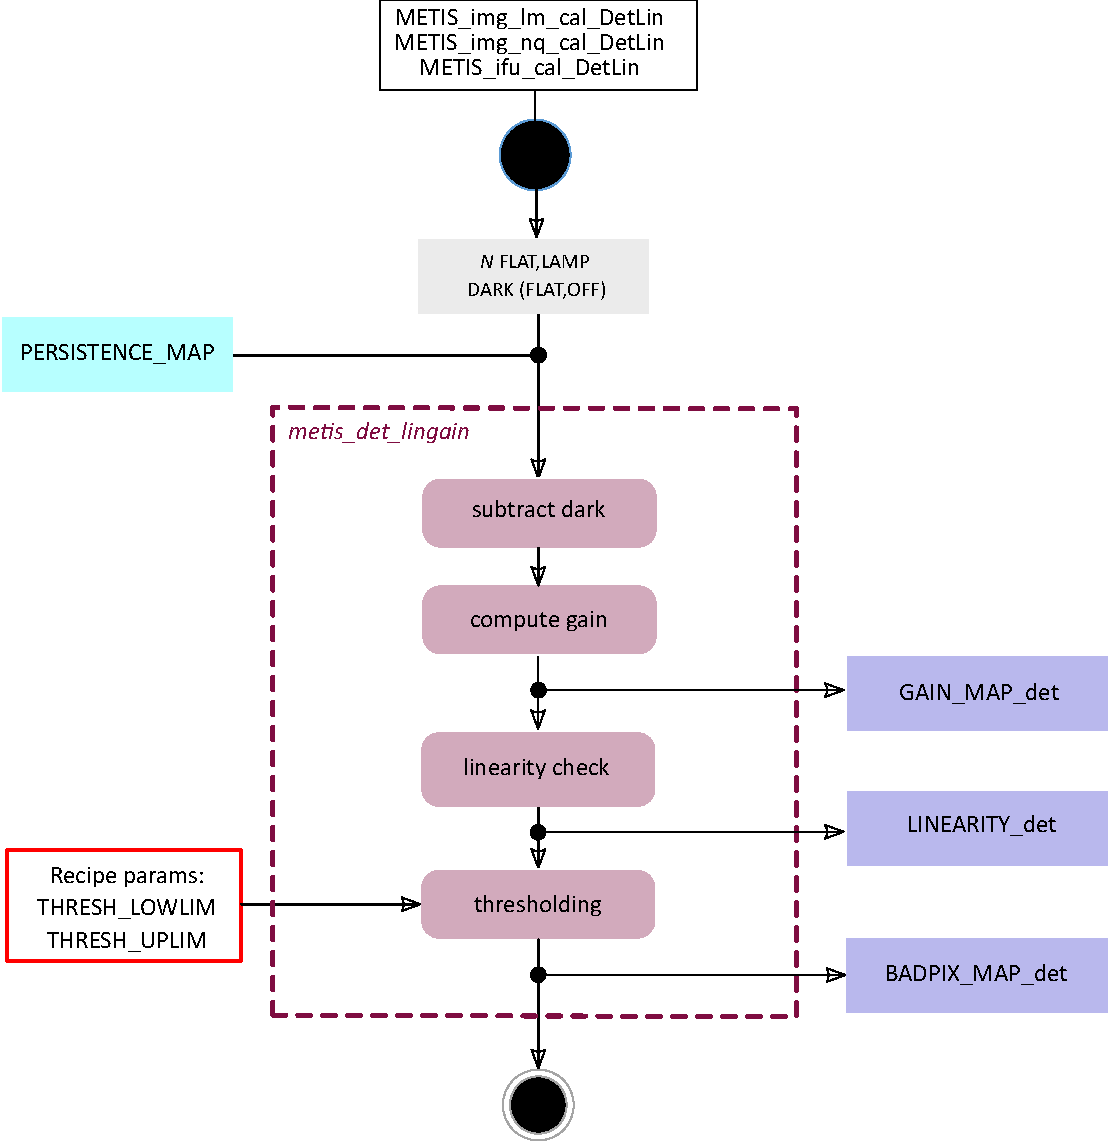
\includegraphics[width=0.65\textwidth]{metis_det_lingain}
  \caption[Recipe: \REC{metis_det_lingain}]{\REC{metis_det_lingain} --
    determination of linearity and gain of the detectors.}
  \label{Fig:rec_det_lingain}
\end{figure}


\clearpage

\subsubsection{Master dark recipe \REC{metis_det_dark}}
\label{sssec:metis_det_dark}
\label{rec:det_dark}
\label{rec:metis_det_dark}

Darks are taken in daytime for all science detectors
\cite{METIS-calibration_plan}. The data will be classified by detector
(e.g.~\FITS{DET.ID} and \FITS{DET.CHIP.ID}) and integration time
(\FITS{DET.DIT}).\footnote{The dark current is not expected to depend on the readout mode of the detectors. Should hardware tests reveal such a dependence, the recipe will be amended to classify on readout mode as well.} There will be ``METIS-dark''
(with the CLOSED position of the CFO-PP1 wheel) and ``Imager-dark''
(with the CLOSED position in the subsystem PP1), to be distinguished
by keyword \TBD. The former will be used for pipeline processing, the
latter for monitoring purposes.

Each set of raw dark frames is processed into a master dark. For the
IFU, both raw frames and master dark have four extensions
corresponding to the four detectors in the focal-plane array. The
recipe also produces bad pixel masks by identifying hot pixels whose
dark current differs significantly (by more than $\pm 5\sigma$) from
the average over the detector.

This fulfills \REQ{METIS-6063}.

\begin{recipedef}
  Name:                & \hyperref[rec:metis_det_dark]{\REC{metis_det_dark}}                                                        \\
  Purpose:             & determine the dark current of the detectors                                 \\
  Requirements:        & \REQ{METIS-6063}                                                            \\
  Type:                & Calibration                                                                 \\
  Templates:           & \TPL{METIS_gen_cal_dark}                                                    \\
                       & \TPL{METIS_gen_cal_InsDark}                                                 \\
  Input data:          & \hyperref[dataitem:linearity_det]{\STATCALIB{LINEARITY_det}}  \\
                       & \hyperref[dataitem:persistence_map]{\EXTCALIB{PERSISTENCE_MAP}}  \\
                       & \hyperref[dataitem:dark_det_raw]{\EXTCALIB{DARK_det_RAW}}  \\
  Parameters:          & Combination method (\texttt{median}, \texttt{mean},
                         \texttt{sigclip},\dots)                                                  \\
                       & Parameters for combination methods                                          \\
                       & Thresholds for deviant-pixel identification                                      \\
  Algorithm:           & Group files by detector and \texttt{DIT}, based on header keywords           \\
                       & Call function \DRL{metis_determine_dark} for each set of files\\
                       & Compute median or average of input frames to improve statistics.            \\  % separate routine, or part of determine dark
                       & call \DRL{metis_update_dark_mask} to flag deviant pixels \\
  Output data:         & \hyperref[dataitem:master_dark_det]{\PROD{MASTER_DARK_det}}                                                      \\
% The BPM_COLD_det and BPM_HOT_det do not seem to add value that BADPIX_MAP_det
% does not already provide. Furthermore, the COLD/HOT specific items are not
% otherwise used in the design, so it seems simpler to just remove them.
%                       & \hyperref[dataitem:bpm_cold_det]{\PROD{BPM_COLD_det}}                                                         \\
%                       & \hyperref[dataitem:bpm_hot_det]{\PROD{BPM_HOT_det}}                                                          \\
                       & \hyperref[dataitem:badpix_map_det]{\PROD{BADPIX_MAP_det}}                                                          \\
  Expected accuracies: & 0.1\% (cf. \cite{METIS_calerrbudget})                                          \\
  QC1 parameters:      & \QC{QC DARK MEAN}                                                              \\
                       & \QC{QC DARK MEDIAN}                                                            \\
                       & \QC{QC DARK RMS}                                                               \\
                       & \QC{QC DARK NBADPIX}                                                             \\
                       & \QC{QC DARK NCOLDPIX}                                                               \\
                       & \QC{QC DARK NHOTPIX}                                                                \\
                       & (more \TBD)                                                                  \\
  hdrl functions:      & \CODE{hdrl_bpm_3d_compute}                                 \\
                       & \CODE{hdrl_imagelist_collapse}                             \\
\end{recipedef}

\begin{figure}[hb]
  \centering
    \begingroup
        \def \globalscale {0.700000}
        \fontsize{10}{12}\selectfont
        % % Document preamble. Comment out for final figure! Footer too!
% \documentclass[tikz, margin=5mm, dvipsnames]{standalone}
% \usepackage{listings}
% 
% ADDING NEW DEFINITIONS -------------------------------------------- start
\definecolor{listingbg}{gray}{0.95}
\definecolor{darkgreen}{rgb}{0.0, 0.7, 0.0}
\definecolor{darkblue} {rgb}{0.0, 0.0, 0.7}
\definecolor{cyan} {rgb}{0.0, 0.4, 0.4}
\definecolor{darkred}  {rgb}{0.7, 0.0, 0.0}
\definecolor{darkorange}{rgb}{1.0, 0.49, 0.0}
\definecolor{violett}{rgb}{255, 0, 255}
\definecolor{turq}{rgb}{0.0, 0.7, 0.8}
\definecolor{fits}{rgb}{0.4, 0.1, 1}


\makeatletter
\lstdefinestyle{RAWstyle}{%
  basicstyle=\ttfamily\color{black}%
  \lst@ifdisplaystyle\scriptsize\fi}

\lstdefinestyle{PARstyle}{%
  basicstyle=\ttfamily\color{black}%
  \lst@ifdisplaystyle\scriptsize\fi}

\lstdefinestyle{DRLstyle}{%
  basicstyle=\ttfamily\color{black}%
  \lst@ifdisplaystyle\scriptsize\fi}

\lstdefinestyle{RECstyle}{%
  basicstyle=\ttfamily\color{black}%
  \lst@ifdisplaystyle\scriptsize\fi}

\lstdefinestyle{QCstyle}{%
  basicstyle=\ttfamily\color{black}%
  \lst@ifdisplaystyle\scriptsize\fi}

\lstdefinestyle{TPLstyle}{%
  basicstyle=\ttfamily\color{black}%
  \lst@ifdisplaystyle\scriptsize\fi}

\lstdefinestyle{PRODstyle}{%
  basicstyle=\ttfamily\color{black}%
  \lst@ifdisplaystyle\scriptsize\fi}

\lstdefinestyle{EXTCALIBstyle}{%
  basicstyle=\ttfamily\color{black}%
  \lst@ifdisplaystyle\scriptsize\fi}

\lstdefinestyle{STATCALIBstyle}{%
  basicstyle=\ttfamily\color{black}%
  \lst@ifdisplaystyle\scriptsize\fi}
\makeatother

% \makeatletter
\newcommand{\replaceunderscores}[1]{\expandafter\replace@underscores#1_\relax}

\def\replace@underscores#1_#2\relax{%
    \ifx \relax #2\relax
        #1%
    \else
        #1%
        \textunderscore
        \replace@underscores#2\relax
    \fi
}

\ExplSyntaxOn
% Generic \Smart@Item macro:
%   use \NEWRAW*{WHATEVER_THIS_IS} where hyperlinks are not needed (TOC, sections...)
%   and \NEWRAW{WHATEVER_THIS_IS} for a full hyperlink-enabled version in regular text and tikz figures
\NewDocumentCommand{\Smart@Item}{m m m O{dataitem}}{%
    \IfBooleanTF{#1}{%
        \texorpdfstring{\lstinline[style=#2style]!#3!}{\replaceunderscores{#3}}%
    }{%
        \hyperref[#4:\text_lowercase:n{#3}]{\lstinline[style=#2style]!#3!}%
    }%
}
\ExplSyntaxOff

% Raw FITS file: \NEWRAW{LM_SCI_RAW}
\NewDocumentCommand{\NEWRAW}{s m}{\Smart@Item{#1}{RAW}{#2}}
\NewDocumentCommand{\NEWPAR}{s m}{\Smart@Item{#1}{PAR}{#2}}
\NewDocumentCommand{\NEWDRL}{s m}{\Smart@Item{#1}{DRL}{#2}}
\NewDocumentCommand{\NEWREC}{s m}{\Smart@Item{#1}{REC}{#2}[rec]}
\NewDocumentCommand{\NEWQC}{s m}{\Smart@Item{#1}{QC}{#2}}
\NewDocumentCommand{\NEWTPL}{s m}{\Smart@Item{#1}{TPL}{#2}}
\NewDocumentCommand{\NEWPROD}{s m}{\Smart@Item{#1}{PROD}{#2}}
\NewDocumentCommand{\NEWREQ}{s m}{\Smart@Item{#1}{REQ}{#2}}
\NewDocumentCommand{\NEWEXTCALIB}{s m}{\Smart@Item{#1}{EXTCALIB}{#2}}
\NewDocumentCommand{\NEWSTATCALIB}{s m}{\Smart@Item{#1}{STATCALIB}{#2}}
\NewDocumentCommand{\NEWFITS}{s m}{\Smart@Item{#1}{FITS}{#2}}
\makeatother

%% Write DRL functions names like this: \hyperref[drl:function]{\DRL{function}}
\newcommand{\RAW}[1]{ \texorpdfstring{\lstinline[style=RAWstyle]!#1!}%
                                     {\replaceunderscores{#1}}}

%% Write DRL functions names like this: \hyperref[drl:function]{\DRL{function}}
\newcommand{\PAR}[1]{ \texorpdfstring{\lstinline[style=PARstyle]!#1!}%
                                     {\replaceunderscores{#1}}}

%% Write DRL functions names like this: \hyperref[drl:function]{\DRL{function}}
\newcommand{\DRL}[1]{ \texorpdfstring{\lstinline[style=DRLstyle]!#1!}%
                                     {\replaceunderscores{#1}}}

%% Write recipe names like this: \REC{metis_do_stuff}
\newcommand{\REC}[1]{ \texorpdfstring{\lstinline[style=RECstyle]!#1!}%
                                     {\replaceunderscores{#1}}}

%% Write QC parameters like this: \QC{QC_SOMETHING_OR_OTHER}
\newcommand{\QC}[1]{ \texorpdfstring{\lstinline[style=QCstyle]!#1!}%
                                    {\replaceunderscores{#1}}}

%% Write templates like this: \TPL{DARK_LM}
\newcommand{\TPL}[1]{ \texorpdfstring{\lstinline[style=TPLstyle]!#1!}%
                                     {\replaceunderscores{#1}}}

%% Write products like this: \hyperref[dataitem:some_thing]{\PROD{SOME_THING}}
\newcommand{\PROD}[1]{ \texorpdfstring{\lstinline[style=PRODstyle]!#1!}%
                                      {\replaceunderscores{#1}}}

%% Write requirements like this: \REQ{METIS-xxxx}
\newcommand{\REQ}[1]{\href{https://polarion.astron.nl/polarion/\#/project/METIS/workitem?id=#1}{\textcolor{brown}{#1}}}

%% external calib files
\newcommand{\EXTCALIB}[1]{ \texorpdfstring{\lstinline[style=EXTCALIBstyle]!#1!}%
                                          {\replaceunderscores{#1}}}

% static calib files
\newcommand{\STATCALIB}[1]{ \texorpdfstring{\lstinline[style=STATCALIBstyle]!#1!}%
                                           {\replaceunderscores{#1}}}

%% Write FITS keywords (and values) like this: \FITS{EXPTIME}
\newcommand{\FITS}[1]{ \texorpdfstring{\lstinline[]!#1!}%
                                      {\replaceunderscores{#1}}}


% \begin{document}


% ADDING NEW DEFINITIONS -------------------------------------------- start
\definecolor{listingbg}{gray}{0.95}
\definecolor{darkgreen}{rgb}{0.0, 0.7, 0.0}
\definecolor{darkblue} {rgb}{0.0, 0.0, 0.7}
\definecolor{cyan} {rgb}{0.0, 0.4, 0.4}
\definecolor{darkred}  {rgb}{0.7, 0.0, 0.0}
\definecolor{darkorange}{rgb}{1.0, 0.49, 0.0}
\definecolor{violett}{rgb}{255, 0, 255}
\definecolor{turq}{rgb}{0.0, 0.7, 0.8}
\definecolor{fits}{rgb}{0.4, 0.1, 1}


\makeatletter
\lstdefinestyle{RAWstyle}{%
  basicstyle=\ttfamily\color{black}%
  \lst@ifdisplaystyle\scriptsize\fi}

\lstdefinestyle{PARstyle}{%
  basicstyle=\ttfamily\color{black}%
  \lst@ifdisplaystyle\scriptsize\fi}

\lstdefinestyle{DRLstyle}{%
  basicstyle=\ttfamily\color{black}%
  \lst@ifdisplaystyle\scriptsize\fi}

\lstdefinestyle{RECstyle}{%
  basicstyle=\ttfamily\color{black}%
  \lst@ifdisplaystyle\scriptsize\fi}

\lstdefinestyle{QCstyle}{%
  basicstyle=\ttfamily\color{black}%
  \lst@ifdisplaystyle\scriptsize\fi}

\lstdefinestyle{TPLstyle}{%
  basicstyle=\ttfamily\color{black}%
  \lst@ifdisplaystyle\scriptsize\fi}

\lstdefinestyle{PRODstyle}{%
  basicstyle=\ttfamily\color{black}%
  \lst@ifdisplaystyle\scriptsize\fi}

\lstdefinestyle{EXTCALIBstyle}{%
  basicstyle=\ttfamily\color{black}%
  \lst@ifdisplaystyle\scriptsize\fi}

\lstdefinestyle{STATCALIBstyle}{%
  basicstyle=\ttfamily\color{black}%
  \lst@ifdisplaystyle\scriptsize\fi}
\makeatother

%%% This file contains definitions of shapes and nodes used
%%% for a recipe workflow
%%% Author       : Oliver Czoske
%%% Created      : 2021-03-03
%%% Last Changed : 2021-03-03
%%% Changes:
%%%

\usetikzlibrary{
  shapes.misc,
  positioning,
  calc,
  arrows.meta}

%% All connecting lines have an arrow
\tikzset{
  connection_arrow/.style={->, >=Latex[open], thick}
}

%% Start and stop buttons (black disks, stop with ring)
%% These are pics, use as
%%         \pic (name) [above of=..] {picname};
\tikzset{
  start/.pic = {
    \node (-m) at (0, 0){};
    \filldraw [fill=black] (0, 0) circle (0.2);
  }
}

\tikzset{
  stop/.pic = {
    \node (-m) at (0, 0){};
    \node (-t) at (0, -0.3){};
    \filldraw [fill=black] (0, 0) circle(0.2);
    \draw[black] (0, 0) circle (0.3);
  }
}


%%%% Various boxes and their colours
%%%% These are nodes, use as
%%%% \node (name) [type, location]  {text};

\definecolor{stepcolor}{RGB}{210,169,188}
\definecolor{rawcolor}{RGB}{205,205,205}
\definecolor{externalcolor}{RGB}{183,255,255}
\definecolor{calibcolor}{RGB}{255,250,216}
\definecolor{calproductcolor}{RGB}{185,184,237}
\definecolor{qcproductcolor}{RGB}{255,201,165}
\definecolor{sciproductcolor}{RGB}{197,219,183}
\definecolor{framecolor}{RGB}{127,13,65}

\tikzset{
  %% template : the template(s) that trigger(s) the recipe
  template/.style={
    rectangle,
    draw=black,
    minimum width=4.0cm,
    minimum height=0.5cm,
    align=center
  },
  %% input : the input files
  input/.style={
    rectangle,
    fill=rawcolor,
    minimum width=4.0cm,
    minimum height=0.75cm,
%     text width=3cm,
    align=center
  },
  %% calib : calibration input
  calib/.style={
    rectangle,
    fill=calibcolor,
    minimum width=4.0cm,
    minimum height=0.75cm,
%     text width=3cm,
    align=center
  },
  %% external : external input
  external/.style={
    rectangle,
    fill=externalcolor,
    minimum width=4.0cm,
    minimum height=0.75cm,
%     text width=3.5cm,
    align=center
  },
  %% params : parameters
  params/.style={
    rectangle,
    draw=red,
    thick,
    minimum width=4.0cm,
    minimum height=0.75cm,
%     text width=3cm,
    align=center
  },
  %% redstep : a reduction step
  %%      ("step" is predefined and can't be used)
  redstep/.style={
    rectangle,
    rounded corners=0.2cm,
    fill=stepcolor,   %%% define colour!
    minimum width=4.0cm,
    minimum height=1cm,
%     text width=3cm,
    align=center
  },
  %% connection : connection to input or output
  connection/.style={
    circle,
    fill=black,
    minimum size=0.15cm,
    inner sep=0pt
  },
  %% sciproduct : a science product
  sciproduct/.style={
    rectangle,
    fill=sciproductcolor,
    minimum width=4.0cm,
    minimum height=0.75cm,
%     text width=3.5cm,
    align=center
  },
  %% calproduct : a calibration product
  calproduct/.style={
    rectangle,
    fill=calproductcolor,
    minimum width=4.0cm,
    minimum height=0.75cm,
%     text width=3.5cm,
    align=center
  },
  %% frame : frame around the recipe
  %% This is a path, use as
  %%    \draw [frame] (upper left) rectangle (lower right);
  frame/.style={framecolor, very thick, dashed}
}



\begin{tikzpicture}
  [x=1cm,
  y=-1cm,
  align=center,
  node distance=2cm and 3cm]
  \sffamily

  %% Grid for orientation. Comment out for final figure!
%   \draw[help lines, green](-5, 0) grid (8, 11);

  %% Main reduction flow
  \node (template) [template] {%
    \TPL{METIS_gen_cal_dark}\\
    \TPL{METIS_gen_cal_InsDark}};
  \pic (start) [below=0.75cm of template] {start};
  \node (input) [below=0.75cm of start-m, input] {\textsl{N} \RAW{DARK_det_RAW}};
  \node (step_linearity) [below=2.0cm of input, redstep] {%
    apply non-linearity correction};

  \node (connectlinearity) [connection] at ($(input)!0.65!(step_linearity)$){};
  \node (linearity) [left=of connectlinearity, external]{\STATCALIB{LINEARITY_det}};
  \draw (linearity) -- (connectlinearity);

  \node (step_persistence) [below of=step_linearity, redstep] {%
    apply persistence correction};

  \node (connectpersistence) [connection] at ($(step_linearity)!0.5!(step_persistence)$){};
  \node (persistence) [left=of connectpersistence, external]{\EXTCALIB{PERSISTENCE_MAP}};
  \draw (persistence) -- (connectpersistence);

  \node (step_filtering) [below of=step_persistence, redstep] {%
    per pixel median/ mean filtering};
  \node (step_thresholding) [below of=step_filtering, redstep] {thresholding};
  \pic (stop) [below=2.0cm of step_thresholding] {stop};

  %% Connections
  \draw (template) -- (input);
  \draw (input) -- (step_linearity);
  \draw (step_linearity) -- (step_persistence);
  \draw (step_persistence) -- (step_filtering);
  \draw (step_filtering) -- (step_thresholding);
  \draw (step_thresholding) -- (stop-t);

  %% Output
  \node (connectdark) [connection] at ($(step_filtering)!0.5!(step_thresholding)$){};
  \node (masterdark) [right=of connectdark, calproduct] {\STATCALIB{MASTER_DARK_det}};
  \draw (connectdark) -- (masterdark);

  \node (connecthot) [connection] at ($(step_thresholding)!0.5!(stop-t)$){};
  \node (hot) [right=of connecthot, calproduct] {\STATCALIB{BADPIX_MAP_det}};
  \draw (connecthot) -- (hot);

  %% frame around recipe
  \draw [frame] ($(input)!0.4!(step_linearity) - (2.5cm,0)$)
  rectangle ($(step_thresholding)!0.7!(stop-t) + (2.5cm, 0)$);
  \node [framecolor, anchor=north west] at
  ($(input)!0.4!(step_linearity) - (2.5cm,0)$) {\textsl{metis\_det\_dark}};

\end{tikzpicture}

% ADDING NEW DEFINITIONS -------------------------------------------- start
\definecolor{listingbg}{gray}{0.95}
\definecolor{darkgreen}{rgb}{0.0, 0.7, 0.0}
\definecolor{darkblue} {rgb}{0.0, 0.0, 0.7}
\definecolor{cyan} {rgb}{0.0, 0.4, 0.4}
\definecolor{darkred}  {rgb}{0.7, 0.0, 0.0}
\definecolor{darkorange}{rgb}{1.0, 0.49, 0.0}
\definecolor{violet}{rgb}{255, 0, 255}
\definecolor{turq}{rgb}{0.0, 0.7, 0.8}
\definecolor{fits}{rgb}{0.4, 0.1, 1}


\makeatletter
\lstdefinestyle{RAWstyle}{%
  basicstyle=\ttfamily\color{fits}%
  \lst@ifdisplaystyle\scriptsize\fi}

\lstdefinestyle{PARstyle}{%
  basicstyle=\ttfamily\color{cyan}%
  \lst@ifdisplaystyle\scriptsize\fi}

\lstdefinestyle{DRLstyle}{%
  basicstyle=\ttfamily\color{violet}%
  \lst@ifdisplaystyle\scriptsize\fi}

\lstdefinestyle{RECstyle}{%
  basicstyle=\ttfamily\color{darkgreen}%
  \lst@ifdisplaystyle\scriptsize\fi}

%% Write QC parameters like this: \QC{QC_SOMETHING_OR_OTHER}
\lstdefinestyle{QCstyle}{%
  basicstyle=\ttfamily\color{darkblue}%
  \lst@ifdisplaystyle\scriptsize\fi}

%% Write templates like this: \TPL{DARK_LM}
\lstdefinestyle{TPLstyle}{%
  basicstyle=\ttfamily\color{darkred}%
  \lst@ifdisplaystyle\scriptsize\fi}

%% Write products like this: \hyperref[dataitem:some_thing]{\PROD{SOME_THING}}
\lstdefinestyle{PRODstyle}{%
  basicstyle=\ttfamily\color{darkorange}%
  \lst@ifdisplaystyle\scriptsize\fi}

%% external calib files
\lstdefinestyle{EXTCALIBstyle}{%
  basicstyle=\ttfamily\color{Turquoise}%
  \lst@ifdisplaystyle\scriptsize\fi}

% static calib files
\lstdefinestyle{STATCALIBstyle}{%
  basicstyle=\ttfamily\color{teal}%
  \lst@ifdisplaystyle\scriptsize\fi}
\makeatother


% % Document footer. Comment out for final figure! Header too!
% \end{document}

    \endgroup
  \caption[Recipe: \REC{metis_det_dark}]{\REC{metis_det_dark} -- creation of master
    dark and bad pixel maps}
  \label{Fig:rec_det_dark}
\end{figure}
\clearpage

\subsubsection{Persistence map creation recipe \REC{metis_det_persistence}}
\label{sssec:metis_det_persistence}
\label{rec:metis_det_persistence}

Infrared detectors are prone to persistence due to charges trapped on a variety of timescales. The correction for a given science or
calibration exposure is built from a sequence of exposures preceding the exposure in question. As these may include exposures taken for another proprietary programme, the recipe is run by ESO on data taken from the science archive and its products are again ingested into the archive. The recipe will make use of the \ac{HDRL} function for the creation of the persistence map, which will be provided by \ac{ESO} in the future.\\
We will update this Section as soon as more information is available.

%\begin{recipedef}
%  Name:                & \hyperref[rec:metis_det_persistence]{\REC{metis_det_persistence}}           \\
%  Purpose:             & compute persistence correction maps        \\
%  Requirements:        & \REQ{METIS-9145}                      \\
%  Type:                & Calibration                           \\
%  Templates:           & --                                    \\
%  Parameters:          & \TBD                                  \\
%  Algorithm:           & see hdrl functions:                   \\
%  Output data:         & \hyperref[dataitem:persistence_map]{\PROD{PERSISTENCE_MAP}}                \\
%  Expected accuracies: & \TBD                                  \\
%  QC1 parameters:      & see hdrl functions:                   \\
%  hdrl functions:      & \TBD (\CODE{hdrl_persistence_compute} \\
%\end{recipedef}

%\begin{figure}[hb]
%  \centering
%  \resizebox{0.6\textwidth}{0.1\textwidth}{\TODO{\fbox{Figure to be done}}}
%  \caption[Recipe:
%  \REC{metis_det_persistence}]{\REC{metis_det_persistence} -- creation
%    of persistence correction frames.}
%  \label{Fig:rec_det_persistence}
%\end{figure}

%%%%%%%%%%%%%%%%%%%%%%%%%%%%%%%%%%%%%%%%%%%%%%%%%%%%%%%



%%% Local Variables:
%%% TeX-master: "METIS_DRLD"
%%% End:
